\documentclass[letterpaper,12pt,oneside]{article}

% --- Package Config ---
\usepackage[utf8]{inputenc}         % Character encoding
\usepackage[spanish]{babel}         % Spanish language support
\usepackage{csquotes}               % Recommended by biblatex for babel compatibility
\usepackage{lmodern} % Latin Modern font
\usepackage[T1]{fontenc}          % Codificación de salida de caracteres (obligatorio para copiar bien)

% --- Page Layout and Margins ---
\usepackage{ragged2e}
\usepackage{anysize}                % Flexible margin settings

% \marginsize{3cm}{2.5cm}{1cm}{2cm} % Example: {left}{right}{top}{bottom}

% --- Tables ---
\usepackage{float}                  % Improved table/figure placement
\usepackage{booktabs}               % Professional-quality tables
\usepackage{tabularx}              % Tables with flexible width
\usepackage{longtable}              % Tables spanning multiple pages
\usepackage{array}                  % Extended column definitions
\usepackage{pbox}                   % Line breaks in table cells
\usepackage{colortbl}               % Color in tables

% --- Math ---
\usepackage{amsmath}                % Advanced math typesetting

% --- Graphics and Rotation ---
\usepackage{rotating}               % Rotate tables and figures
\usepackage{pdflscape}              % Landscape pages in PDF

% --- Colors ---
\usepackage{color}                  % Colored text
\definecolor{naranja}{rgb}{1,0.5,0}
\definecolor{rojo}{rgb}{1,0,0}
\definecolor{SteelBlue}{rgb}{0.3,0.5,0.7}

% --- Bibliography ---
\usepackage[style=ieee]{biblatex}   % IEEE bibliography style
\addbibresource{bibliografia.bib}
\usepackage[numbib,notlof,notlot]{tocbibind} % Numbered bibliography in ToC

% --- Hyperlinks ---
\usepackage[pdftex,bookmarks=true,linkcolor=black,citecolor=black,colorlinks=true,urlcolor=black]{hyperref}

% --- Figures and Subfigures ---
\usepackage{subfig}                 % Subfigures
\usepackage{enumitem}               % Customizable lists
\usepackage{url}                    % URL formatting
\usepackage{caption}
\captionsetup{skip=1em, font=small}

% --- Custom Spaces between paragraphs ---
\setlength{\parskip}{1em}
\setlength{\parindent}{0pt}

\begin{document}
\renewcommand{\tablename}{Tabla}
\justifying % Justify text in the document

% ---------- Portada, Contraportada y Resumen ----------
% Avoid magic strings
\newcommand{\titulo}{Migración de la infraestructura de Firebase a AWS en Paralegales}
\newcommand{\subtitulo}{Pasantía en Modalidad de Convenio}
\newcommand{\autor}{Juan Felipe Monsalve Vargas}
\newcommand{\correoDirector}{royer.estrada@correounivalle.edu.co}
\newcommand{\universidad}{Universidad del Valle}
\newcommand{\facultad}{Facultad de Ingeniería}
\newcommand{\escuela}{Escuela de Ingeniería de Sistemas y Computación}
\newcommand{\sede}{Sede (06) Tuluá}
\newcommand{\anio}{2025}

\newcommand\portada{
  \begin{titlepage}
    \begin{center}
      \begin{figure}[h]
        \centering
        
\includegraphics[width=0.1\textwidth]{img/template/univalle-escudo.jpg}
      \end{figure}
      {\bf \titulo }
      \vspace{0.5cm}
      {\bf \subtitulo }
      \vfill
      {\bf \autor }
      \vfill
      {\bf \universidad  \par}
      {\bf \facultad \par}
      {\bf \escuela \par}
      {\bf \sede \par}
      {\bf \anio \par}
    \end{center}
  \end{titlepage}
}

\newcommand\contraportada{
  \begin{titlepage}
    \begin{center}
      {\bf \titulo }
      \vspace{0.5cm}
      {\bf \subtitulo }
      \vfill
      \vfill
      \vfill
      {\bf \autor \par}
      {\bf Código 202160145 \par}
      {\url{ juan.felipe.monsalve@correounivalle.edu.co } \par}
      \vfill
      \vfill
      \vfill
      {Director \par}
      {\bf Ms.C Royer David Estrada Esponda. Ing \par}
      {Profesor de la Escuela de Ingeniería de Sistemas y Computación \par}
      {\url{royer.estrada@correounivalle.edu.co} \par}
      \vfill
      \vfill
      \vfill
      \vfill
      {\bf \universidad  \par}
      {\bf \facultad \par}
      {\bf \escuela \par}
      {\bf \sede \par}
      {\bf \anio \par}
    \end{center}
  \end{titlepage}
}
\portada
\contraportada

\newpage
\section*{Resumen}

Paralegales es una plataforma de legaltech orientada a automatizar el seguimiento de procesos judiciales en la Rama Judicial Unificada en Colombia. El objetivo principal de esta solución es simplificar la tarea de los abogados al ofrecer herramientas que permiten monitorear automáticamente los cambios en los procesos judiciales, además de proporcionar funcionalidades complementarias para mejorar la eficiencia en la gestión legal.

Para acelerar la salida a producción, el desarrollo de Paralegales se hizo uso del Software Development Kit (SDK) de Firebase, lo que permitió avanzar rápidamente en funcionalidades clave. Sin embargo, esta decisión trajo consigo importantes compromisos técnicos, como la implementación de lógica de negocio crítica directamente en el frontend, lo que representa riesgos de seguridad y dificultades para aplicar principios de escalabilidad.

El presente proyecto tiene como objetivo principal migrar y adaptar la infraestructura tecnológica de Paralegales desde Firebase hacia un entorno 100\% en AWS (Amazon Web Services). Esta migración busca mejorar la seguridad del sistema, aumentar la escalabilidad y reducir los costos operativos, además de permitir trasladar lógica de negocio sensible actualmente implementada en el frontend hacia entornos seguros como AWS Lambda.

\hfill

\textbf{Palabras clave:}  Ingeniería de software, Microservicios, Enterprise migration, Cloud computing, APIs, Vendor lock-in, Legaltech.


% ---------- Tablas ----------
\newpage
\renewcommand\contentsname{Tabla de Contenido}
\tableofcontents

\newpage
\renewcommand\listtablename{Lista de tablas}
\listoftables

\newpage
\renewcommand\listfigurename{Lista de Figuras}
\listoffigures

% ---------- Chapters ----------
\section{Introducción}

En Colombia, el acceso a la información judicial se ha centralizado mediante el Portal  “Rama Judicial Unificada”, una página web donde cualquier ciudadano puede consultar el estado de los procesos legales. Sin embargo, este sistema no cuenta con mecanismos automatizados de seguimiento o notificación de cambios, lo cual obliga a los profesionales del derecho a revisar constantemente el estado de cada proceso de forma manual \cite{Paez2024}. Sumado a esto,  según el Consejo Superior de la Judicatura para el 2023 el índice de congestión de la justicia en Colombia fue de 54.9\% \cite{Rozo2024}. Esta situación, especialmente crítica para abogados que gestionan múltiples casos, no solo representa una carga operativa considerable, sino que también incrementa el riesgo de omitir actualizaciones importantes que pueden afectar el desarrollo de los casos.

Ante este panorama, se abre una clara oportunidad de negocio para desarrollar software que automatice y optimice esta tarea, además de ofrecer funcionalidades adicionales que permitan aprovechar este nicho de mercado. Todo esto, de la mano de tecnologías emergentes como la inteligencia artificial, la computación, entre otras. Estas tecnologías permiten no solo reducir la carga operativa del profesional jurídico, sino también mejorar la calidad del servicio prestado al cliente \cite{Botero2023}. En este contexto, el sector \textit{Legaltech} ha ganado tracción en Colombia y Latinoamérica, Siendo Colombia quien ocupa el segundo lugar en cuanto a productos de software en la industria jurídica según el Legal Tech Index \cite{Sierra2023}.

En este marco surge Paralegales, una plataforma desarrollada por la empresa Webcloster S.A.S., cuyo propósito es automatizar el seguimiento de procesos judiciales y brindar a los abogados una experiencia más eficiente, inteligente y centralizada. Este proyecto de grado tiene como objetivo migrar la infraestructura actual de Paralegales, basada parcialmente en Firebase, hacia un entorno 100\% en AWS. Esta migración permitirá mejorar la seguridad de la lógica de negocio, actualmente expuesta en el cliente (\textit{frontend}), aumentar la escalabilidad del sistema y reducir los costos operativos. Además, se buscará aplicar las mejores prácticas de ingeniería de software dentro de lo posible para fortalecer la calidad técnica del producto durante su evolución.

\section{Descripción de la empresa}

\subsection{Descripción General}
Webcloster S.A.S. es una empresa del sector de tecnologías de la información y la comunicación que, en respuesta a las necesidades del entorno, innova en la forma de trabajar y administrar recursos mediante la creación de plataformas tecnológicas de servicios. A través de sus propios sistemas de información, la compañía apoya a organizaciones de todos los tamaños para que puedan alcanzar su máximo potencial mediante las soluciones tecnológicas que ofrece.

\subsection{Misión}
Empresa dedicada a la creación y desarrollo de Software que facilita la gestión y administración efectiva de las operaciones empresariales y personales, brindando soluciones innovadoras que se adaptan a las necesidades de nuestros clientes buscando siempre incrementar la productividad y competitividad con servicios de alto valor agregado, y confiabilidad.

\subsection{Visión}
Establecer un posicionamiento en el sector de las TIC; implementado los cambios que la globalización demande con respecto al desarrollo de software y aplicativos móviles, mejorando continuamente cada uno de los procesos implementados, cumpliendo requerimientos de nuestros clientes y comprometidos de forma transparente con sus necesidades.

\subsection{Valores Corporativos}
\begin{itemize}
  \item \textbf{Honestidad:}  es vital la transparencia y sinceridad.
  \item \textbf{Pasión:} "Disfrutar lo que hacemos"
  \item \textbf{Puntualidad:} Tener especial consideración con el tiempo de clientes, proveedores y jefes.
  \item \textbf{Calidad:} Garantizar los mejores productos y servicios ante el mundo.
  \item \textbf{Trabajo en equipo:} Tolerancia, respeto, admiración, lealtad y solidaridad.
  \item \textbf{Orientación al cliente:} adecuarnos a las necesidades de nuestros clientes.
  \item \textbf{Mejora Continua:} Mejora y revolución de procesos, productos y servicios para aumentar la calidad y satisfacción de resultados de forma sostenible.
  \item \textbf{Resolución de problemas:} Incentivamos el pensamiento de nuestros colaboradores orientado a la búsqueda de soluciones culpables óptimas para mejorar y no buscar
  \item \textbf{Responsabilidad Social:} Causar un impacto amplio y positivo ante la sociedad que nos rodea.
\end{itemize}

% TODO: Organigrama de Webcloster

\section{Formulación del problema}

\subsection{Descripción del problema}
Actualmente, la plataforma Paralegales presenta una serie de problemas estructurales derivados de decisiones técnicas tomadas durante su etapa inicial de desarrollo. Como se aprecia en la \autoref{fig:arbol_problemas}, el principal problema identificado es la exposición de lógica de negocio crítica en el cliente, lo que genera una serie de consecuencias negativas a nivel de seguridad, arquitectura, costos y gestión tecnológica.

Uno de los efectos más graves de esta exposición es el alto riesgo de inseguridad en la plataforma, ya que la lógica sensible puede ser inspeccionada, manipulada o replicada por terceros, lo que constituye un ejemplo de \textit{Insecure Design}, una categoría de riesgo identificada en el OWASP Top 10 \cite{OWASP2021}.

Además, la dependencia de servicios propietarios como Firebase, fenómeno conocido como \textit{vendor lock-in} \cite{OparaMartins2016, OparaMartins2014,Harauzek2022}, genera costos operativos más elevados y compromete la viabilidad económica de la plataforma a largo plazo. Asimismo, la falta de centralización en un único ecosistema tecnológico provoca fragmentación, lo que dificulta la integración, el mantenimiento y la escalabilidad del sistema.

Actualmente, Paralegales utiliza funciones AWS Lambda (\textit{backend}) para manejar algunos casos de uso que requieren lógica crítica del lado del servidor. Sin embargo, mantener lógica crítica tanto en el \textit{frontend} como en el \textit{backend} agrava la fragmentación tecnológica. Desde el punto de vista de diseño de sistemas (\textit{system design}), esta dispersión de componentes críticos genera una arquitectura inconsistente y difícil de escalar y mantener, como se ilustra también en la \autoref{fig:arbol_problemas}.

En la raíz del problema, como se expone en la \autoref{fig:arbol_problemas}, se encuentra la priorización de la velocidad en el desarrollo sobre la adopción de buenas prácticas \cite{BirrEngwall2024}. Esta decisión condujo a una dependencia parcial de Firebase y sus tecnologías propietarias, así como a la omisión de delegar lógica crítica en entornos de ejecución que corren del lado del servidor como AWS Lambda o Cloud Functions, incrementando los riesgos mencionados.

Por lo tanto, se evidencia la necesidad urgente de una reestructuración tecnológica que permita resolver estos problemas, mejorando la seguridad, reduciendo costos, y garantizando una arquitectura sólida y escalable para el futuro del proyecto.

\newcommand\captionArbolProblemas{Árbol de problemas.\hspace{1em}}

\begin{figure}[H]
  \centering
  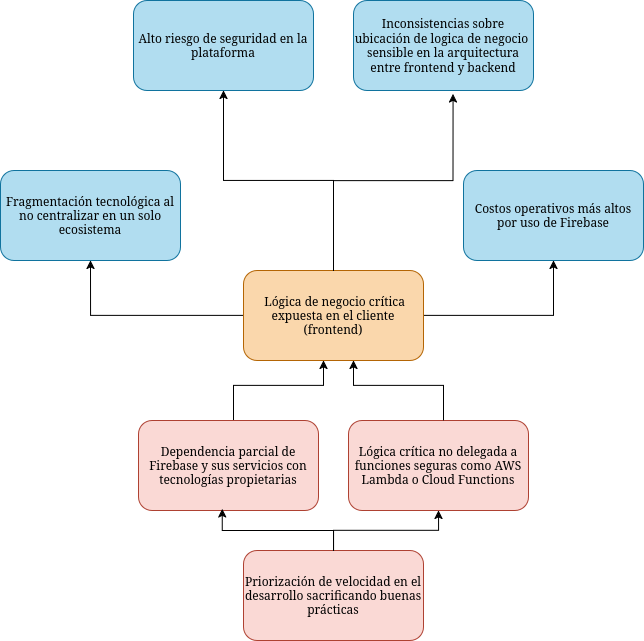
\includegraphics[width=0.85\textwidth]{img/figures/fig2-arbol-de-problemas.png}
  \caption[\captionArbolProblemas]{\captionArbolProblemas Fuente: Elaboración Propia.}
  \label{fig:arbol_problemas}
\end{figure}

\subsection{Definición del Problema}
A partir del análisis realizado, se plantea como problema central a resolver el siguiente:
\begin{quote}
  \textbf{¿Cómo migrar y adaptar la infraestructura de la plataforma Paralegales desde Firebase hacia AWS de manera que se mejore la seguridad, se elimine la exposición de lógica crítica en el cliente, se reduzcan los costos operativos y se optimice la escalabilidad y mantenibilidad del sistema?}
\end{quote}

De este problema principal se derivan las siguientes preguntas específicas:

\begin{enumerate}
  \item \textbf{¿Qué servicios de AWS pueden reemplazar adecuadamente los servicios actuales de Firebase utilizados en Paralegales?}
  \item \textbf{¿Qué estrategias de migración permiten trasladar de forma segura y eficiente tanto los datos almacenados en la base de datos como los registros de usuarios desde Firebase hacia AWS, minimizando el impacto operativo?}
  \item \textbf{¿Cómo puede estructurarse una arquitectura basada en AWS que mejore la seguridad y reduzca la fragmentación tecnológica?}
  \item \textbf{¿Qué enfoques técnicos y metodológicos deben adoptarse durante el proceso de migración para garantizar la integridad de los datos y la continuidad del servicio?}
  \item \textbf{¿Qué medidas deben tomarse para optimizar los costos en AWS sin comprometer la calidad del servicio?}
\end{enumerate}

Estas preguntas guiarán el desarrollo del proyecto y permitirán estructurar un plan de migración que no solo atienda las necesidades actuales, sino que también prepare a la plataforma para un crecimiento seguro y sostenible.


% ----------Referencias----------
\newpage
\printbibliography
\nocite{*}

\end{document}

% TODO: debe estar justificado